\newcommand{\RNum}[1]{\uppercase\expandafter{\romannumeral #1\relax}}

\chapter{Theory}\label{ch:theory}
In the following, a fundamental overview of the theoretical background needed to understand the results of this thesis is given. First, the basics of magnetism and FMR are explained, followed by an introduction to spin pumping. After that, a general introduction to superconductivity is provided. Finally, basic concepts of lithography are discussed.

\section{Fundamentals of Magnetism}
\subsection{Macrospin Model}
The magnetic properties of a ferromagnet without local defects or domains can be best described by treating the ferromagnet as having one average magnetic dipole. This average dipole, called Magnetization $\mathbf{M}$, can then be calculated by the sum of all dipole moments $\boldsymbol{\mu}$ of a sample:
\begin{equation}    
\mathbf{M} = \frac{1}{V}\sum_{i\in V}{\boldsymbol{\mu_\textbf{i}}}
\end{equation}
From classical electrodynamics, we know that the magnetic dipoles $\boldsymbol{\mu}$ are related to the angular momentum $\textbf{L}$ by the gyromagnetic ratio $\gamma$, due to the electron creating a current through its orbital path:
\begin{equation}
   \boldsymbol{\mu} = \gamma \textbf{L} 
   \label{Drehimpulsgleichung}
\end{equation}
Furthermore, when a magnetic field $\mathbf{B}$ is applied to a magnetic dipole moment $\boldsymbol{\mu}$, it causes a torque $\textbf{T}$ on the dipole moment:
\begin{equation}
    \textbf{T} = \boldsymbol{\mu} \times \mathbf{B}
    \label{Drehmoment von dipolmoment}
\end{equation}
By using equations (\ref{Drehimpulsgleichung}) and (\ref{Drehmoment von dipolmoment}), as well as the fact that $\textbf{T} = \diff{\textbf{L}}{t}$, we obtain the following equation of motion for a dipole moment $\boldsymbol{\mu}$:
\begin{equation}
    \diff{\boldsymbol{\mu}}{t} = \gamma \boldsymbol{\mu} \times \mathbf{B} 
    \label{EOM fuer dipolmoment}
\end{equation}
Inside a magnetized medium, the magnetic flux density takes on the following form \cite{obstbaum2014}:
\begin{equation} 
\textbf{B} = \mu_0(\textbf{H+M}),
\end{equation}
where $\textbf{H}$ is the applied magnetic field. To transfer this result to the dynamics of the magnetization of a medium, equation (\ref{EOM fuer dipolmoment}) has to be reformulated in such a way that it accounts for the effective field $\mathbf{{H_{\text{eff}}}}$ inside the medium. Doing this, we get the Landau-Lifschitz equation \cite{obstbaum2014}:
\begin{equation}
    \diff{\textbf{M}}{t} = - \gamma \textbf{M} \times \mu_0 \mathbf{{H_{\text{eff}}}}
    \label{Landau-Lifschitz}
\end{equation}
Here, $\mathbf{{H_{\text{eff}}}}$ combines all possible field terms inside the medium, such as anisotropy $\mathbf{H_{\text{ani}}}$ and the demagnetizing field $\mathbf{H_{\text{dem}}}$ \cite{obstbaum2014}.
Solving this differential equation leads to a magnetization undergoing precession around the effective field with the frequency $ \omega = \gamma \mu_0 H_{\text{eff}}$ \cite{Mueller2019}, as shown in figure \ref{fig:precession picture}.

In a real physical system, however, the precession amplitude declines due to various dissipation effects such as magnon-phonon relaxation or radiative damping. Gilbert therefore introduced a damping term with the material-dependent coefficient $\alpha$ with which we get the Landau-Lifschitz-Gilbert (LLG) equation \cite{Liensberger2021}
\begin{equation}
    \diff{\textbf{M}}{t} = - \gamma \textbf{M} \times \mu_0 \mathbf{{H_{\text{eff}}}} + \frac{\alpha}{M_s}\mathbf{M} \times\diff{\textbf{M}}{t},
\end{equation}
where $M_s$ refers to the saturation magnetization, which is the maximum magnetization a ferromagnetic material can achieve.

\subsection{Ferromagnetic Resonance}
In order to investigate the resonance condition of this precession, we introduce an oscillating magnetic driving field $\mathbf{h_{\text{rf}}}$ that is perpendicular to $\mathbf{{H_{\text{eff}}}}$. $\mathbf{h_{\text{rf}}}$ can generate a torque that can compensate the damping of the precession when the frequency of the magnetization precession and the frequency of the oscillating field match, which can be described by a driven harmonic oscillator in the classical view \cite{Liensberger2021}.
The following derivation will closely follow references \cite{Liensberger2017} and \cite{Mueller2019}. We choose our coordinate system so that the external magnetic field $\mathbf{{H_{\text{ext}}}}$ is applied in the $z$-axis and $\mathbf{h_{\text{rf}}}$ rotates in the $xy$-plane. We split $\textbf{H}_\textrm{eff}$ and $\textbf{M}$ into their respective time-independent and time-dependent parts 
\begin{equation}
    \begin{aligned}
        \mathbf{M} &= \mathbf{M}_0 + \mathbf{m}(t) = M_0 \mathbf{\hat{e}}_z + \mathbf{m}(t) \\
        \mathbf{H}_{\text{eff}} &= \mathbf{H}_{\text{ext}} - \mathbf{H}_{\text{dem}} + \mathbf{h}_{\text{rf}}(t) \\
        &= (H_{\text{ext}} - N_z M_0) \mathbf{\hat{e}}_z - N_x m_x(t) \mathbf{\hat{e}}_x - N_y m_y(t) \mathbf{\hat{e}}_y + \mathbf{h}_{\text{rf}}(t) 
    \end{aligned}
    \label{time-dependent and independent}
\end{equation}
where $N_{x/y/z}$ denote the terms from the demagnetization tensor (note that this description of the magnetization is only applicable if the precession angle is small). For simplicity, the anisotropy field is neglected, since during the course of this thesis, only samples with Ni$_{80}$Fe$_{20}$, also known as Permalloy, were studied, which does not have a structural anisotropy \cite{Decker_2017}. For the oscillating magnetic field $\mathbf{h_{\text{rf}}}$ and $\textbf{m}(t)$, we use a harmonic ansatz:
\begin{equation}
\begin{aligned}
\mathbf{h}_{\text{rf}}(t) &= (h_{\text{rf},x}, h_{\text{rf},y}, 0)^{\text{T}} \cdot e^{i\omega t} \\
\mathbf{m}(t) &= (m_{x}, m_{y}, 0)^{\text{T}} \cdot e^{i\omega t}
\label{harmonic ansatz}
\end{aligned}
\end{equation}

By plugging in equations (\ref{time-dependent and independent}) and (\ref{harmonic ansatz}) into the LLG-equation, we can derive the resonance condition
\begin{equation}
\omega_\text{res} = \gamma\mu_0 \sqrt{\left[H_{\text{ext}} + H_\textrm{shift} + (N_x - N_z) \cdot M_s\right]\left[H_{\text{ext}} + H_\textrm{shift} + (N_y - N_z) \cdot M_s\right]}
\label{Kittel equation}
\end{equation}
which is known as the Kittel equation. Here, $H_\textrm{shift}$ is the shift in the resonance field that occurs due to the superconductor focusing magnetic flux onto the ferromagnet, a phenomenon that is further discussed in chapter \ref{ch:results}. If the magnetic field $H_{\text{ext}}$ is applied in the plane of the sample, the equation can be further simplified to:
\begin{equation}
\omega_\text{res} = \gamma \mu_0 \sqrt{(H_{\text{ext}} + H_\textrm{shift})(H_{\text{ext}} + H_\textrm{shift} +M_\text{s})}
\end{equation}
Additionally, the derivation gives us an equation for the resonance line width $\Delta H_{\textrm{FWHM}}$, as a function of the driving frequency and the damping coefficient \cite{Mueller2023}:
\begin{equation}
    \Delta H_{\textrm{FWHM}} = \Delta H_0 + \frac{\alpha \omega}{\mu_0 \gamma}
    \label{linewidth equation}
\end{equation}
where $\alpha$ is the Gilbert-damping coefficient and $\Delta H_0$ the line width offset that comes from extrinsic mechanisms.

The response of the magnetization to the oscillating magnetic field $\mathbf{h_{\text{rf}}}$ can be described by the complex magnetic susceptibility $\chi = \chi' + i\chi''$ (Polder susceptibility), where $\chi'$ is the real part describing dispersion and $\chi''$ the imaginary part describing absorption. The relation between the perpendicular magnetization $\mathbf{m}$ and $\mathbf{h_{\text{rf}}}$ is given by $ \mathbf{m} = \chi \mathbf{h_{\text{rf}}}$ \cite{Liensberger2017}. An example plot of the Polder susceptibility can be seen in figure \ref{fig:Polder}.

\begin{figure}[htbp] % [htbp] for flexible placement
    \centering % Center the entire figure
    \begin{subfigure}[c]{0.48\textwidth} % Adjust width for 3 subfigures
        \subcaption{} % Place (a) above the image
        \centering
        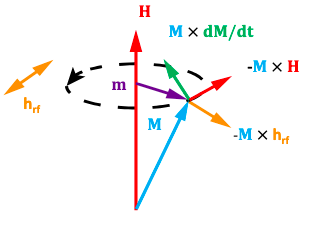
\includegraphics[width=\linewidth,height = 6cm]{chapters/Photos/Theory/Landau-Lifschitz Precession.png}
        \label{fig:precession picture}
    \end{subfigure}
    \hfill % Flexible horizontal space
    \begin{subfigure}[c]{0.48\textwidth} % Adjust width for 3 subfigures
        \subcaption{} % Place (b) above the image
        \centering
        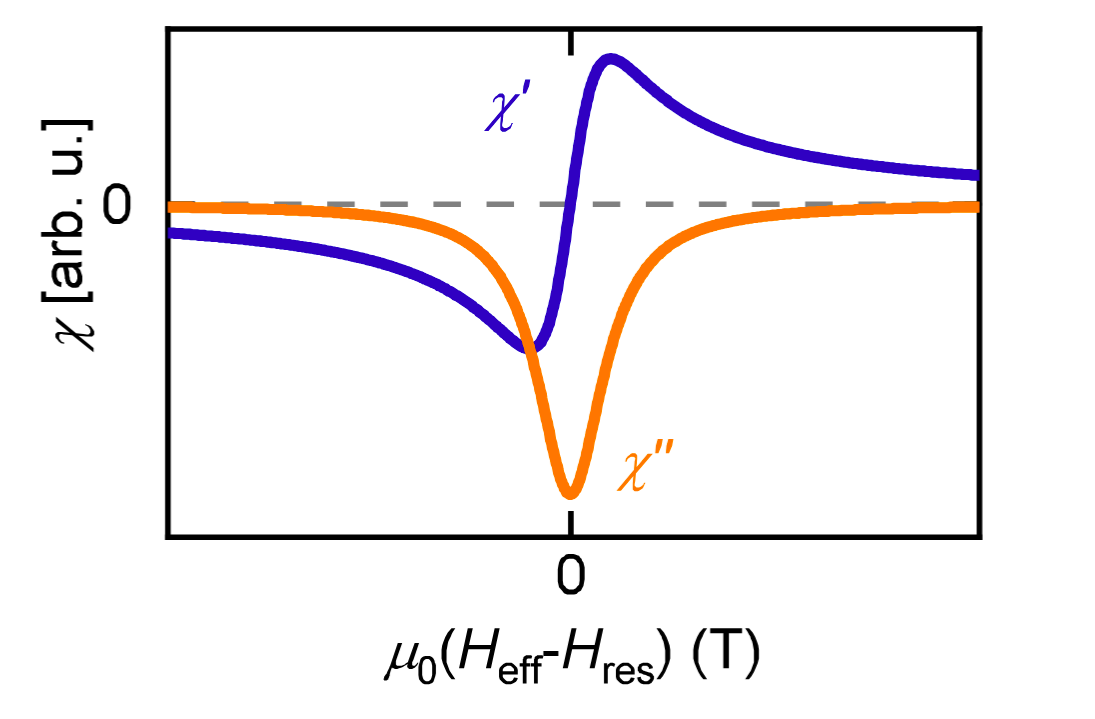
\includegraphics[width=\linewidth, height = 6cm]{chapters/Photos/Theory/FMR_example.png} % Assuming you have a third image here for (b)
        \label{fig:Polder}
    \end{subfigure}
    \hfill % Flexible horizontal space
    \caption{(a): Schematic model showing the precession of the magnetization $\textbf{M}$ of the medium around the effective field $\mathbf{{H_{\text{eff}}}}$. (b) : Example plot of the Polder susceptibility, where $\chi$' is the real part showing dispersion and $\chi$'' the imaginary part showing absorption. The perpendicular magnetization $\textbf{m}$ in (a) is related to $\mathbf{h_{\text{rf}}}$ by the equation $\textbf{m} = \chi \mathbf{h_{\text{rf}}}$. The images were taken from \cite{Liensberger2017}.}
    \label{fig:ferromagnetic_resonance} % Main label for the entire figure
\end{figure}






\subsection{Spin Pumping}
\begin{figure}[htbp]
    \centering
    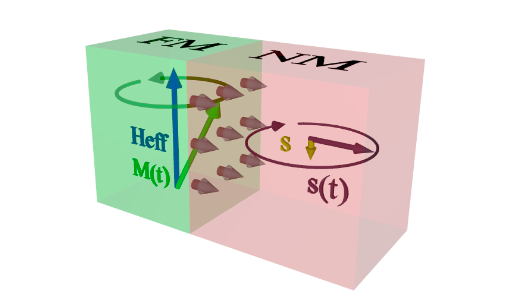
\includegraphics[width=0.5\linewidth]{chapters/Photos/Theory/spin pumping.png}
    \caption{Example illustration of spin pumping from a ferromagnet (FM) to a normal metal (NM). The spin current is depicted as gray arrows on the interface, whereas $\textbf{s}$ and $\mathbf{s(\text{t})}$ are the DC- and AC-parts of the polarization vector, respectively. Taken from \cite{obstbaum2014}.}
    \label{fig:enter-label}
\end{figure}

When a ferromagnetic film comes in contact with a normal metal, an increase in damping is observed, which is known as spin pumping. Theoretically, this can be explained by a spin current $\mathbf{J_\textbf{s}}$ that gets sent across the ferromagnet/metal interface which transports angular momentum from the ferromagnet to the normal metal, hence increasing the damping. The spin current density is given by \cite{Mueller2023}
\begin{equation}
\mathbf{J}_{\mathbf{s}}=\frac{\hbar}{4 \pi}\left(\operatorname{Re}\left(G_{\uparrow \downarrow}\right) \mathbf{M} \times \frac{d \mathbf{M}}{d t}-\operatorname{Im}\left(G_{\uparrow \downarrow}\right) \frac{d \mathbf{M}}{d t}\right)
\end{equation}
where $G_{\uparrow \downarrow}$ is the spin-mixing conductance that describes the transport of spins that are not collinear to the magnetization of the sample. The first term corresponds to a damping-like behavior, and the second term gives a field-like contribution. The imaginary part of the spin-mixing conductance is typically negligible ~\cite{obstbaum2014}. The additional contribution in damping is then given by 
\begin{align*}
    \alpha_{\textrm{sp}} =& \ \frac{g\mu_0}{4 \pi M_S}\frac{G_{\uparrow \downarrow}}{d_{\text{FM}}}
\end{align*}
where $g$ is the Landé-Factor and $d_\textrm{FM}$ the thickness of the ferromagnet \cite{Mueller2023}. Studying ferromagnet/normal metal samples at different thicknesses of the ferromagnet can be done to examine its effects on the Gilbert-damping. Together with the intrisic damping $\alpha_0$ of the ferromagnet, the total damping is then given by $\alpha = \alpha_0 + \alpha_{\textrm{sp}}$.

The main objective of this bachelor thesis was to investigate how the thickness of the superconductor influences the spin-transport through it. Therefore, the spin pumping effect is of great importance.

\section{Fundamentals of Superconductivity}
In this section, the fundamental theory behind superconductivity is discussed that is needed for the discussion of the results given in chapter \ref{ch:results}.

Superconductors are materials that exhibit two distinct properties below a critical temperature $T_\textrm{C}$: The vanishing of electrical resistance and the expulsion of the magnetic field inside the material, also called the Meißner effect. In its essence, superconductivity is caused by a positive attraction of two electrons through an exchange of virtual phonons. Intuitively, this can be explained by an electron moving through the crystal, causing a deformation in the lattice that generates a dipole moment, which in turn attracts another electron. The two electrons have opposite momentum $\mathbf{k}$ and $\mathbf{-k}$ and form so-called Cooper pairs \cite{Hunklinger2018}. 

\subsection{The London equations}
In 1935, the London brothers developed the London equations in an attempt to phenomenologically explain the behavior of superconductors. To derive these equations, one needs to start with the Drude model and the relation 
\begin{equation}
    m\diff{\textbf{v}}{t} = -q\textbf{E} - m\frac{d\mathbf{v_{\textrm{d}}}}{dt}.
\end{equation}
Since there is no electrical resistance during superconductance, the second term vanishes. By using $\mathbf{j_s} = n q \textbf{v}$, one can derive the first London equation \cite{Hunklinger2018}
\begin{equation}
    \frac{\partial\mathbf{j_s}}{\partial t} \ = \  \frac{nq^2}{m}\textbf{E} 
    \label{first London equation}
\end{equation}
where $n$ represents the Cooper pair density, $m$ the mass and $q$ the charge of a Cooper pair.
Inserting (\ref{first London equation}) into the Maxwell-equation $\nabla \times \mathbf{E} = -\frac{\partial \mathbf{B}}{\partial t}$ yields
\begin{equation}
    \diff{}{t}(\nabla \times \mathbf{j_s} + \frac{nq^2}{m}\textbf{B}) = 0.
    \label{d/dt of second london equation}
\end{equation}
Since not only the time derivative of the magnetic flux, but the magnetic flux itself vanishes in a superconductor, the London brothers argued that the equation inside the derivative must also vanish, leading to the second London equation \cite{Hunklinger2018}
\begin{equation} 
    \nabla \times \mathbf{j_s} = -\frac{nq^2}{m}\textbf{B}
    \label{second London equation}
\end{equation}
Solving these equations yields 
\begin{align}
    \mathbf{B(}\textbf{r}) =& \mathbf{B_\textrm{0}}e^{-\frac{|r|}{\lambda_L}},
\end{align}
where $\lambda_L$ = $\frac{m}{\mu_0 nq^2}$ is the London penetration depth \cite{Mueller2019}. It measures how deep a magnetic field will penetrate into the superconductor. 
\subsection{Types of superconductors}
Not all superconductors (SCs) have the same properties, however. SCs can be divided into type-$\RNum{1}$ and type-$\RNum{2}$ SCs. Type-$\RNum{1}$ SCs exhibit the Meißner effect below their critical field $B_\textrm{C}$. Comparatively, a type-$\RNum{2}$ SC has two critical fields, $B_{\textrm{C1}}$ and $B_{\textrm{C2}}$. Below the critical field $B_{\textrm{C1}}$, a type-$\RNum{2}$ SC displays the same properties as a type-$\RNum{1}$ SC. Between $B_{\textrm{C1}}$  and $B_{\textrm{C2}}$, however, type-$\RNum{2}$ SCs create canals that let flux penetrate into the material. Each canal, also called vortex, allows exactly one quantum flux $\Phi$. The vortices usually arrange themselves in a triangular lattice, called the Abrikosov-lattice \cite{Mueller2019}. An illustration of a type-$\RNum{2}$ SC with vortices can be seen in figure \ref{fig:vortices}.

The different behavior between type-$\RNum{1}$ and type-$\RNum{2}$ SCs can be understood when considering the Ginzburg-Landau parameter $\kappa$:
\begin{equation}
    \kappa = \frac{\lambda_{L}}{\xi_{GL}}
\end{equation}

where $\xi_{GL}$ is the Ginzburg-Landau coherence length, which determines how quickly the Cooper pair density increases near the surface. When $\kappa < \frac{1}{\sqrt{2}}$, the SC behaves like a type-$\RNum{1}$ SC, and if $\kappa > \frac{1}{\sqrt{2}}$, the SC is a type-$\RNum{2}$ SC. 
Intuitively, this can be understood as a fight between two opposing effects: Maximizing the surface area minimizes the amount of energy needed to expel magnetic flux from going into the material. At the same time, surfaces reduce the gain of condensation energy, since there are less Cooper pairs near the surface. For type-$\RNum{2}$ SCs, it is more favorable to create small vortices and which costs condensation energy from Cooper pairs, but save on the expulsion energy against the magnetic field \cite{Hunklinger2018}. These vortices often are bound to defects in the material. Lorentz forces caused by current flowing through the SC can cause the vortices to move, which creates dissipation and ultimately destroys the superconducting state \cite{shi2025lorentz}, which is why type-$\RNum{2}$ SCs are often intentionally created with defects to pin the vortices in place. Even with these defects, vortices can jump from defect to defect given enough thermal energy, a phenomenon known as vortex creeping \cite{Eley_2017}.
\begin{figure}
    \centering
    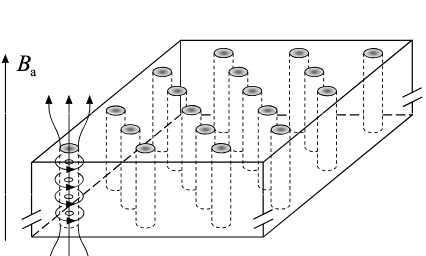
\includegraphics[width=0.5\linewidth]{chapters/Photos/Theory/vortices.png}
    \caption{Sample illustration of vortices in a type-$\RNum{2}$ superconductor. The field lines of the magnetic flux and the currents are depicted for one vortex. Taken from \cite{Hunklinger2018}.}
    \label{fig:vortices}
\end{figure}

\section{Lithography}
Photolithography, or optical lithography, refers to the process of creating structures on a sample by applying a photosensitive polymer material called photoresist (or often abbreviated to resist) and then locally exposing it to light, often in the ultraviolet wavelengths \cite{Mack2006LithographyOnline}. Electron Beam Lithography (EBL), on the other hand, uses high-energy electrons to gain the same effect. In this thesis, optical lithography as well as EBL is used to form structures on the sample and to create an unremovable isolation layer.

\subsection{Typical photolithography process}
Typically, a lithography process involves several steps. These are: Applying the photoresist onto the sample via spin coating, heating it (also called prebake), applying a mask, and exposing the photoresist to UV light. Masks can be omitted by using maskless aligners (MLA), which exposes the photoresist locally by a focused laser. Light exposure changes the solubility of the photoresist: Exposed regions of a positive photoresist become more soluble in the developer, while those of a negative photoresist become less soluble \cite{AllresistPhotoresistOnline}. Developing the sample washes the soluble part off, creating a pattern on the sample that can be used to etch away specific parts of the sample or deposit new material, thus fabricating structures. Finally, the remaining photoresist can be washed away with a remover. When a new material is deposited onto the sample, the material which lies on the photoresist gets washed away along with the photoresist, which is known as lift-off. A sample illustration can be seen in figure \ref{fig:photolithography}.

\begin{figure}
    \centering
    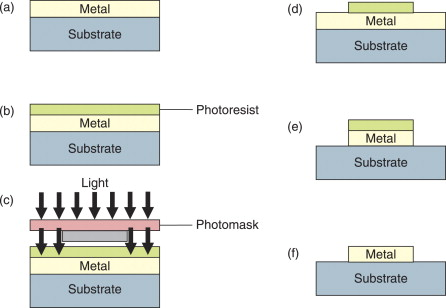
\includegraphics[width=0.7\linewidth]{chapters/Photos/Theory/Photolithography.jpg}
    \caption{Illustration of the positive photolithography process. (a) A metal layer is deposited onto the substrate. (b) A photoresist is then applied onto the sample via spincoating. (c) The photoresist is exposed to UV light through a mask. (d) The sample is developed, removing the resist on the exposed areas. (e) The metal is etched away, while the resist protects the metal beneath it. (f) The remaining photoresist is removed, leaving the metal structure on the substrate. Taken from \cite{sciencedirect_photolithography}.}
    \label{fig:photolithography}
\end{figure}

\subsection{Cross-linking}
Negative photoresists achieve high chemical resistance upon exposure by a process called cross-linking. Cross-linking refers to the reaction where individual polymers chain together to build a single, large polymer, changing the property of the material \cite{AllresistPhotoresistOnline}. In the $\textit{AR-N 1407.17 new}$ (AR-N) negative photoresist, which was used in our experiments, this is done by radical starters that form reactive radicals upon exposure to UV light or high energy electrons, which starts a chain reaction connecting individual polymers together. In this thesis, cross-linking was used to create an isolation layer to prevent electrical contact between the coplanar waveguide (CPW) and the DC contacts, as further explained in chapter \ref{ch:Microfabrication}.
